%Chapter 11


\chapter{Delta \textDelta}\label{ch:Delta}


\lettrine{A}{l}though I promised to move on to extrinsic/time value, first we are going to cover Delta. Delta is an option “Greek”- one of the variables named after letters in the Greek alphabet that defines an option’s behavior. Delta is closely related to moneyness, and is one of the most important options “Greeks” for selling calls, next to theta.

Learning how “the Greeks” function mathematically isn't necessary for trading in a retail account, but the general dynamics of how things move and why they move is invaluable. Although it is somewhat complex at first glance, delta is useful as a concept because it allows you to understand how the price of your sold call changes as the price of the shares you sold it against changes.

Delta will show up in the options chain on your broker’s website, so I snipped this data from 11/22/19 for a preclinical biotech company trading at \$9.81 a share.

\begin{figure}[h!]
  \centering
    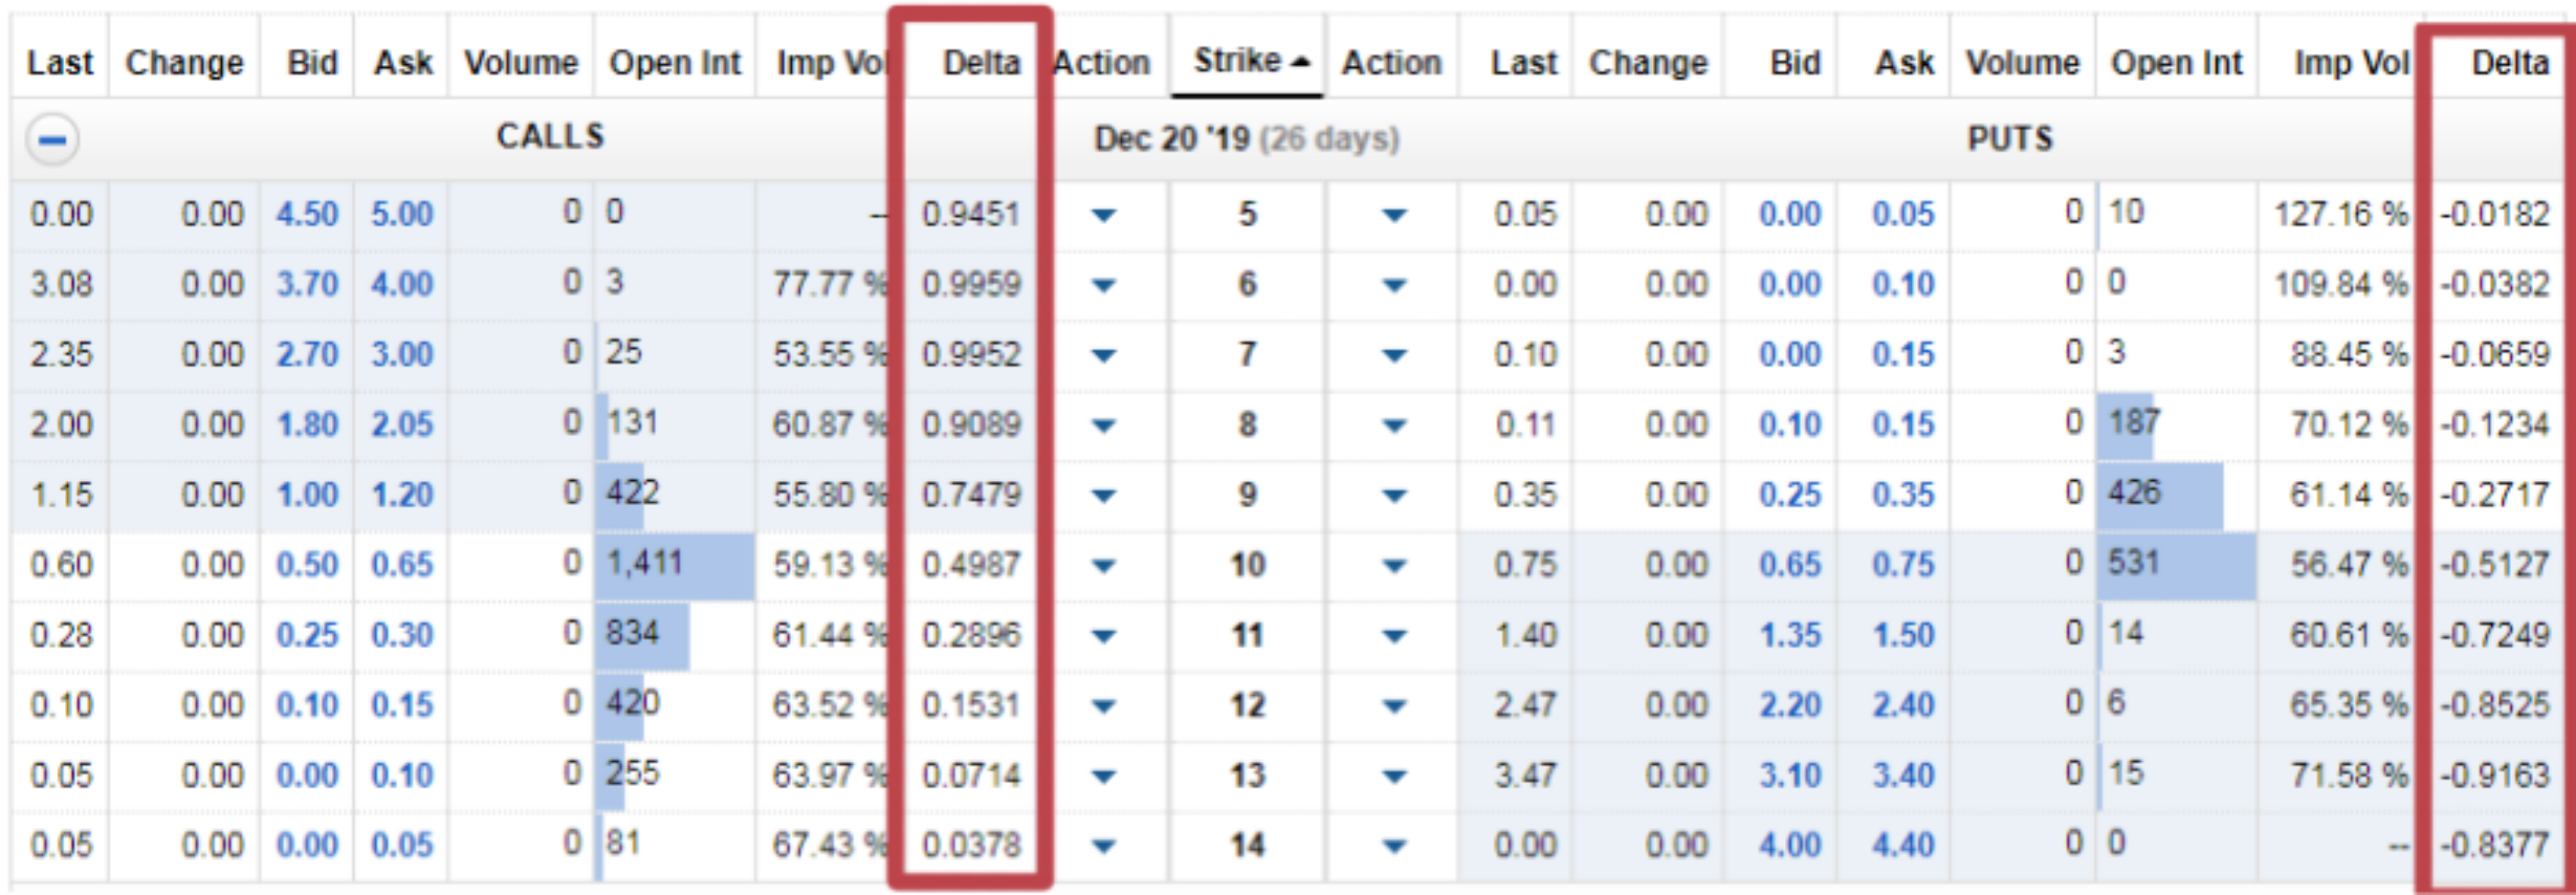
\includegraphics[width=\textwidth]{Images/Ch11/chapter11pic2.png}
    \caption{\emph{Right now the tiny numbers aren't important- I'm simply showing you delta exists.}}
\end{figure}

\section{So What is Delta?}

\begin{center}
\fbox
{
\begin{minipage}{0.90\textwidth}
    \textbf{Delta represents how much the price of an option’s premium will change if the underlying stock\\ appreciates \$1.} 
\end{minipage}
} 
\end{center}

To get your confidence up, just start by knowing that the absolute value of delta will only ever be between zero and one. Its range is limited to 0-1. Easy, right? Since an option price would never move more than the price of the underlying moved, delta is never going to be more than 1. 

For Example: If the delta of a long call option is 0.5 and the underlying investment rises \$1 in price, the price of a long call would go up \$0.50 (50 cents per share). If the delta of a long call is 0.3\footnote{To add some confusion, often a delta is referred to as it's actual value multiplied by 100, so a 0.5 delta may be called the “fifty delta" or a 0.30 delta call referred to as the  “30 delta call". It's just easier to say than “point five zero."} and the price of the underlying drops \$1, the price of the long call would be expected to decrease 30 cents. To reinforce this concept via comparison, stocks have delta=1 (because if the price of a stock moves \$1...the price of the stock moves \$1).

\section{Delta as an Option’s\\ “Responsiveness”}

Another way to think of Delta is as a value that tells you how “sensitive” an option price is to the movement of the underlying stock- the higher the delta, the more the option “responds” to the stock’s price moves.\footnote{For the mathematically inclined, delta is a first-order derivative of stock price (just like acceleration is a derivative of velocity, if you’re into physics).}  Put another way, options with a high delta move whenever the stock moves. Low delta options don't really give a damn what the stock is doing. 


So why is Delta high or low in the first place? What determines whether the option price cares when the price of the underlying moves? Moneyness and implied volatility.

First, we can think about Moneyness. How deep ITM (In-The-Money) or OTM the option is makes the biggest impact on Delta. The easiest way to start understanding is with an example of the farthest OTM option in the chain from before. Zoom in!

\begin{figure}[h!]
  \centering
    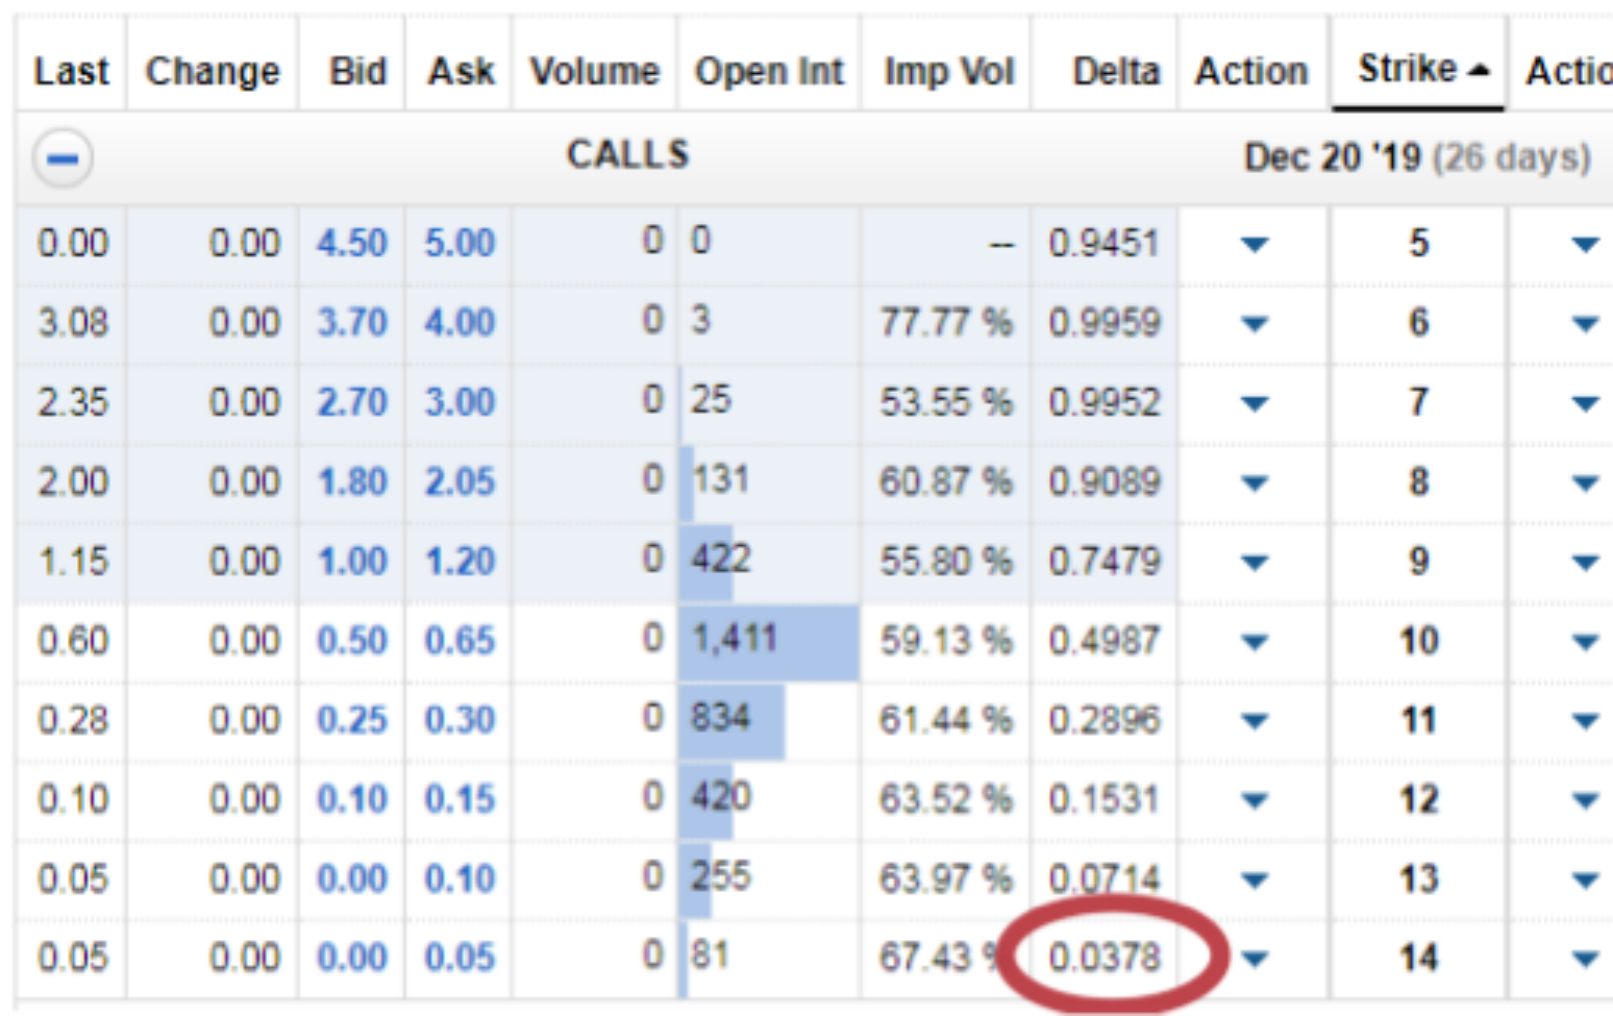
\includegraphics[width=\textwidth]{Images/Ch11/chapter11pic3.png}
\end{figure}

\newpage
Looking at the previous chain, the delta for the \$14 strike call is 0.0378, so for every dollar the stock moves, the price of the \$14 call will increase only 3.78 cents. For example, we bought a \$14 strike call for \$0.05 and the price of the stock increased from \$9.81 to \$10.81, our option premium would theoretically increase by 3.78 cents, from 0.05 to 0.08 cents. 

\begin{figure}[h!]
  \centering
    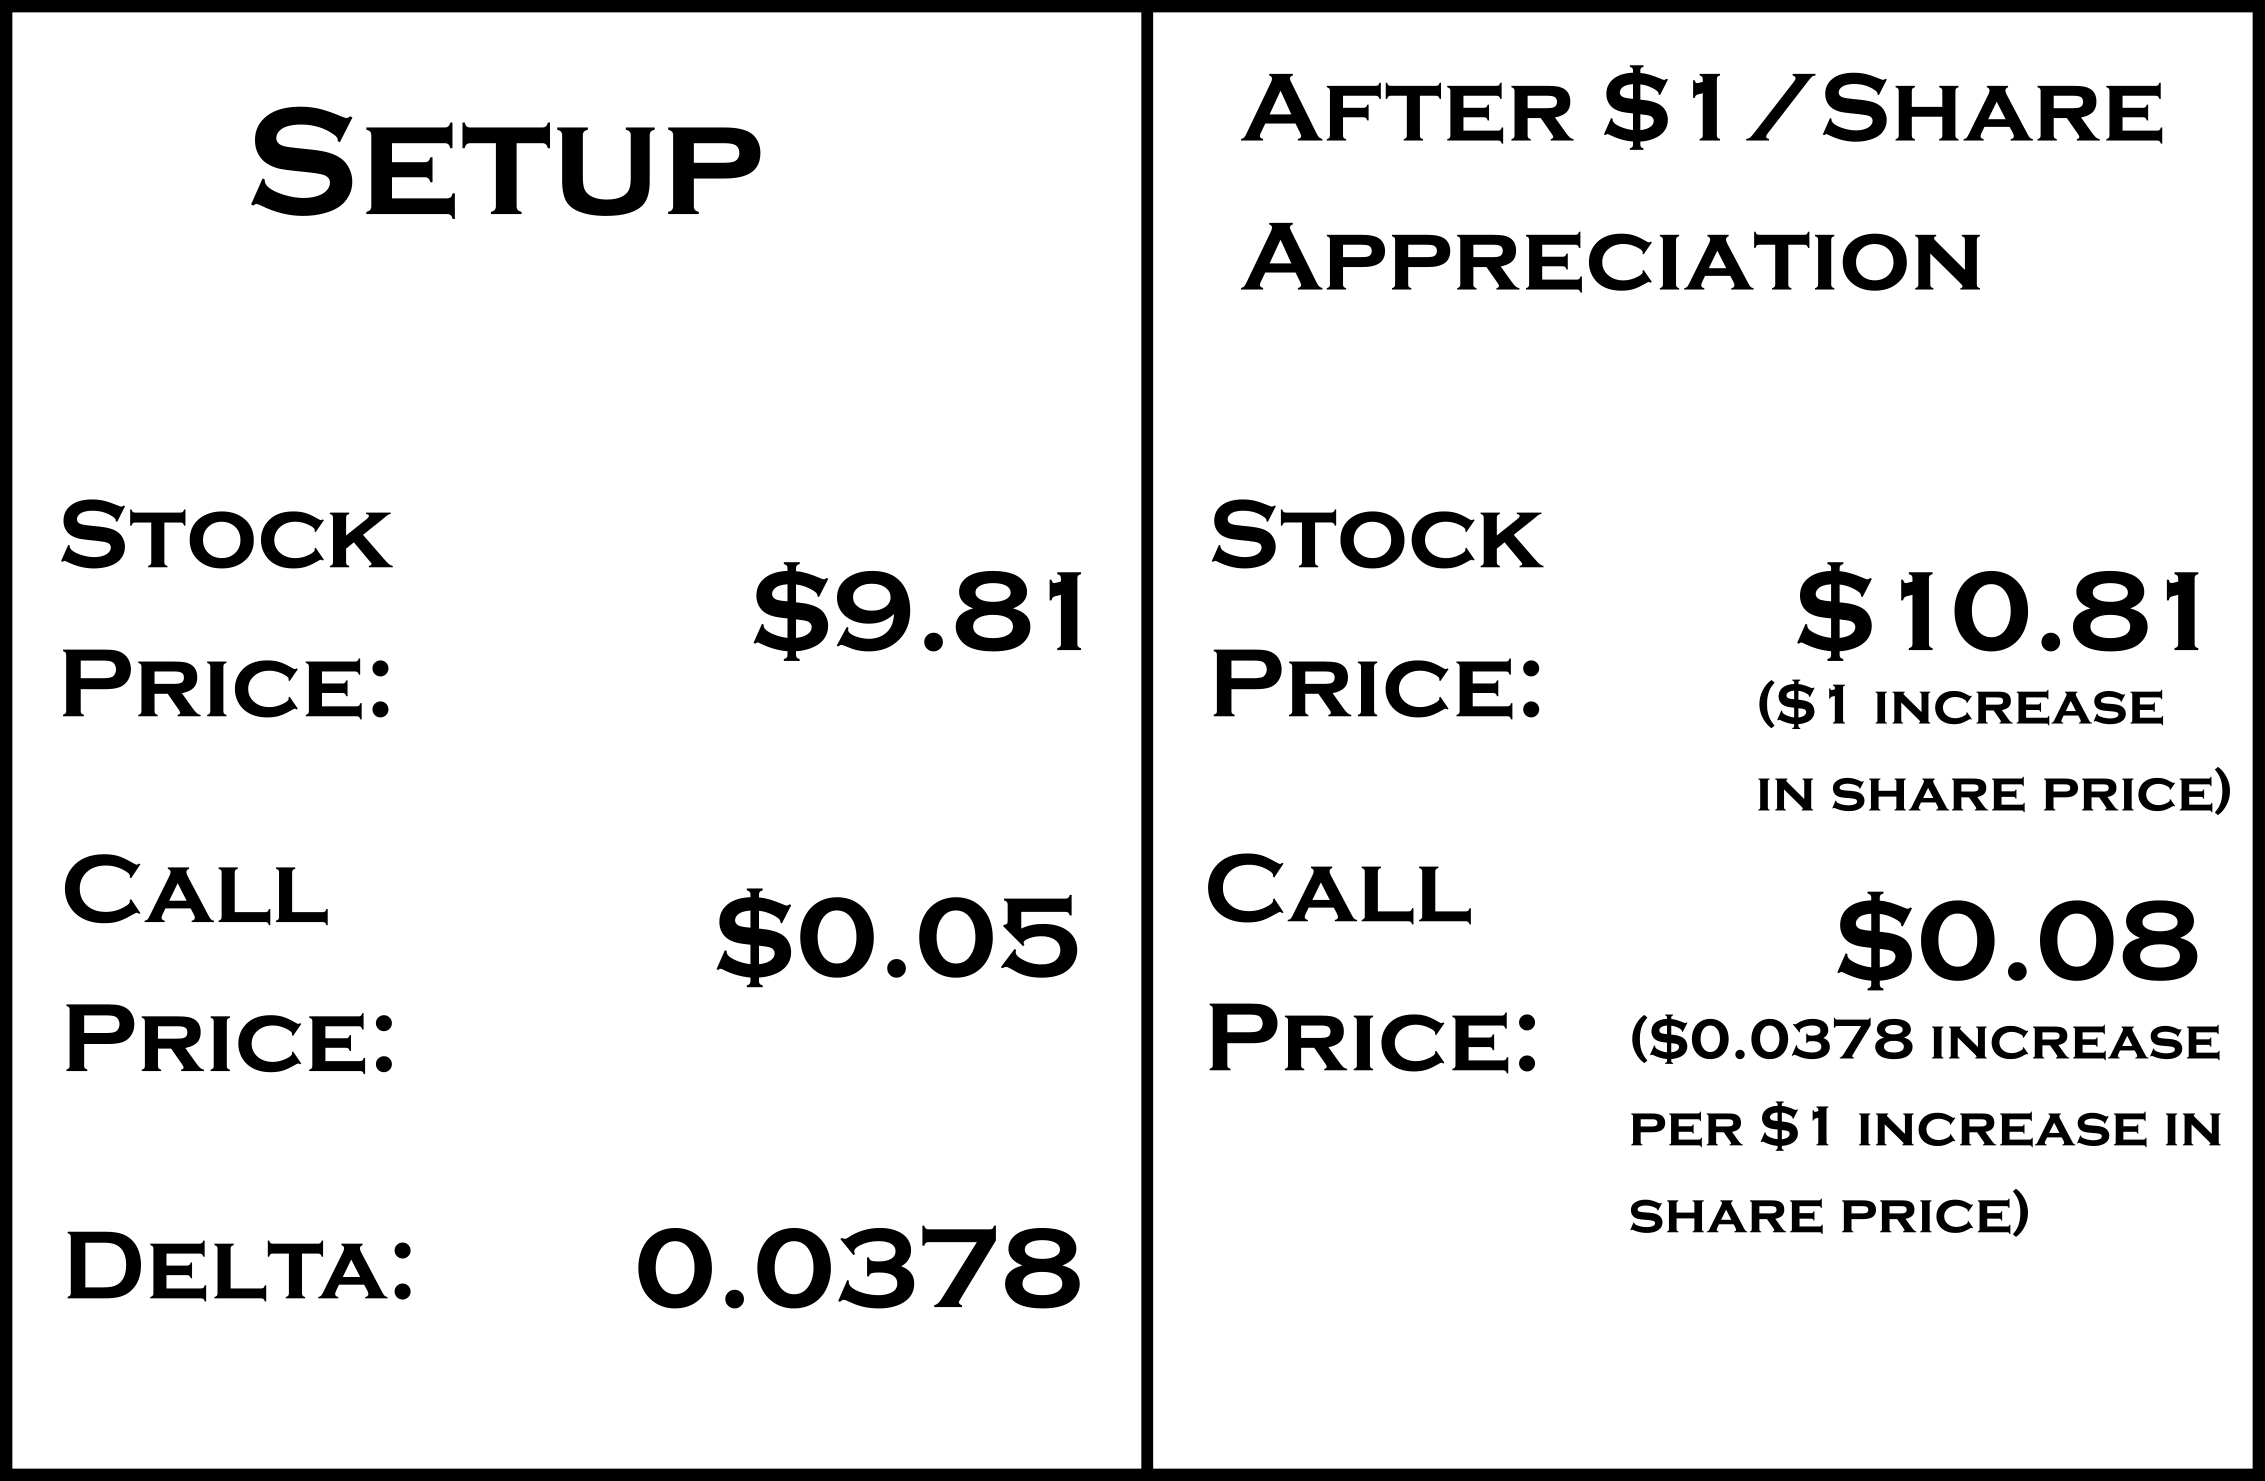
\includegraphics[width=0.85\textwidth]{Images/Ch11/chapter11pic4.png}
\end{figure}

I have to stop right here and say that you need to take this with a huge grain of salt- this understanding is correct in principle, but it doesn’t actually work that way. Delta is more dynamic in practice- you’ll immediately see why in the next chapter: Delta, A Moving Target.

\newpage
But what about a higher delta? If you look at the \$10 strike and \$9 strike options, there is a pretty big jump in delta- it goes from 0.4987 to 0.7479: 

\begin{figure}[H]
  \centering
    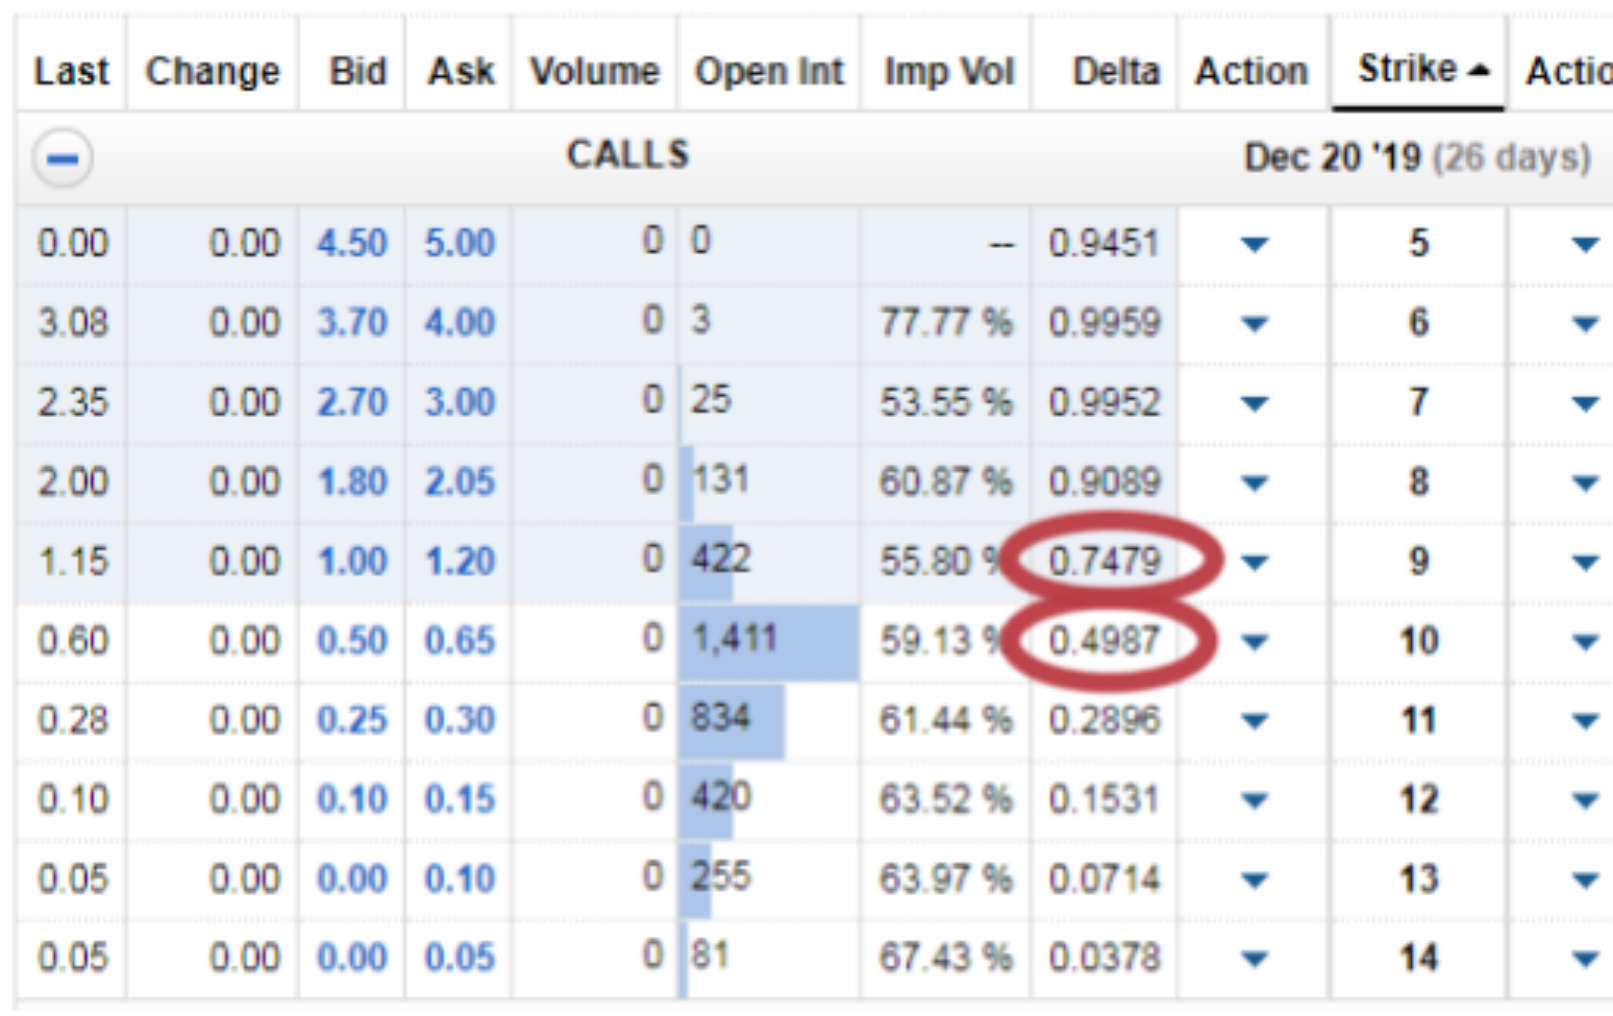
\includegraphics[width=\textwidth]{Images/Ch11/chapter11pic5.png}
\end{figure}

Why the big jump, and for that matter, why do the lower strike calls have a delta that gets closer and closer to 1? Again the reason is the moneyness, aka the intrinsic value. The \$9 call is selling for \$1.15, and since the stock is \$9.81, you know that call has an intrinsic value of \$0.81 cents per share. 

Put another way, if you spent \$1.15 for that call, it is worth at least \$0.81 based on the stock price alone. If the stock goes up \$1 to \$10.81, your call is going to be worth more as well...not one dollar more, but theoretically 74.79 cents more based on the \emph{current} delta (again, take this with a huge grain of salt- you’ll see why in the next chapter).

\begin{figure}[h!]
  \centering
    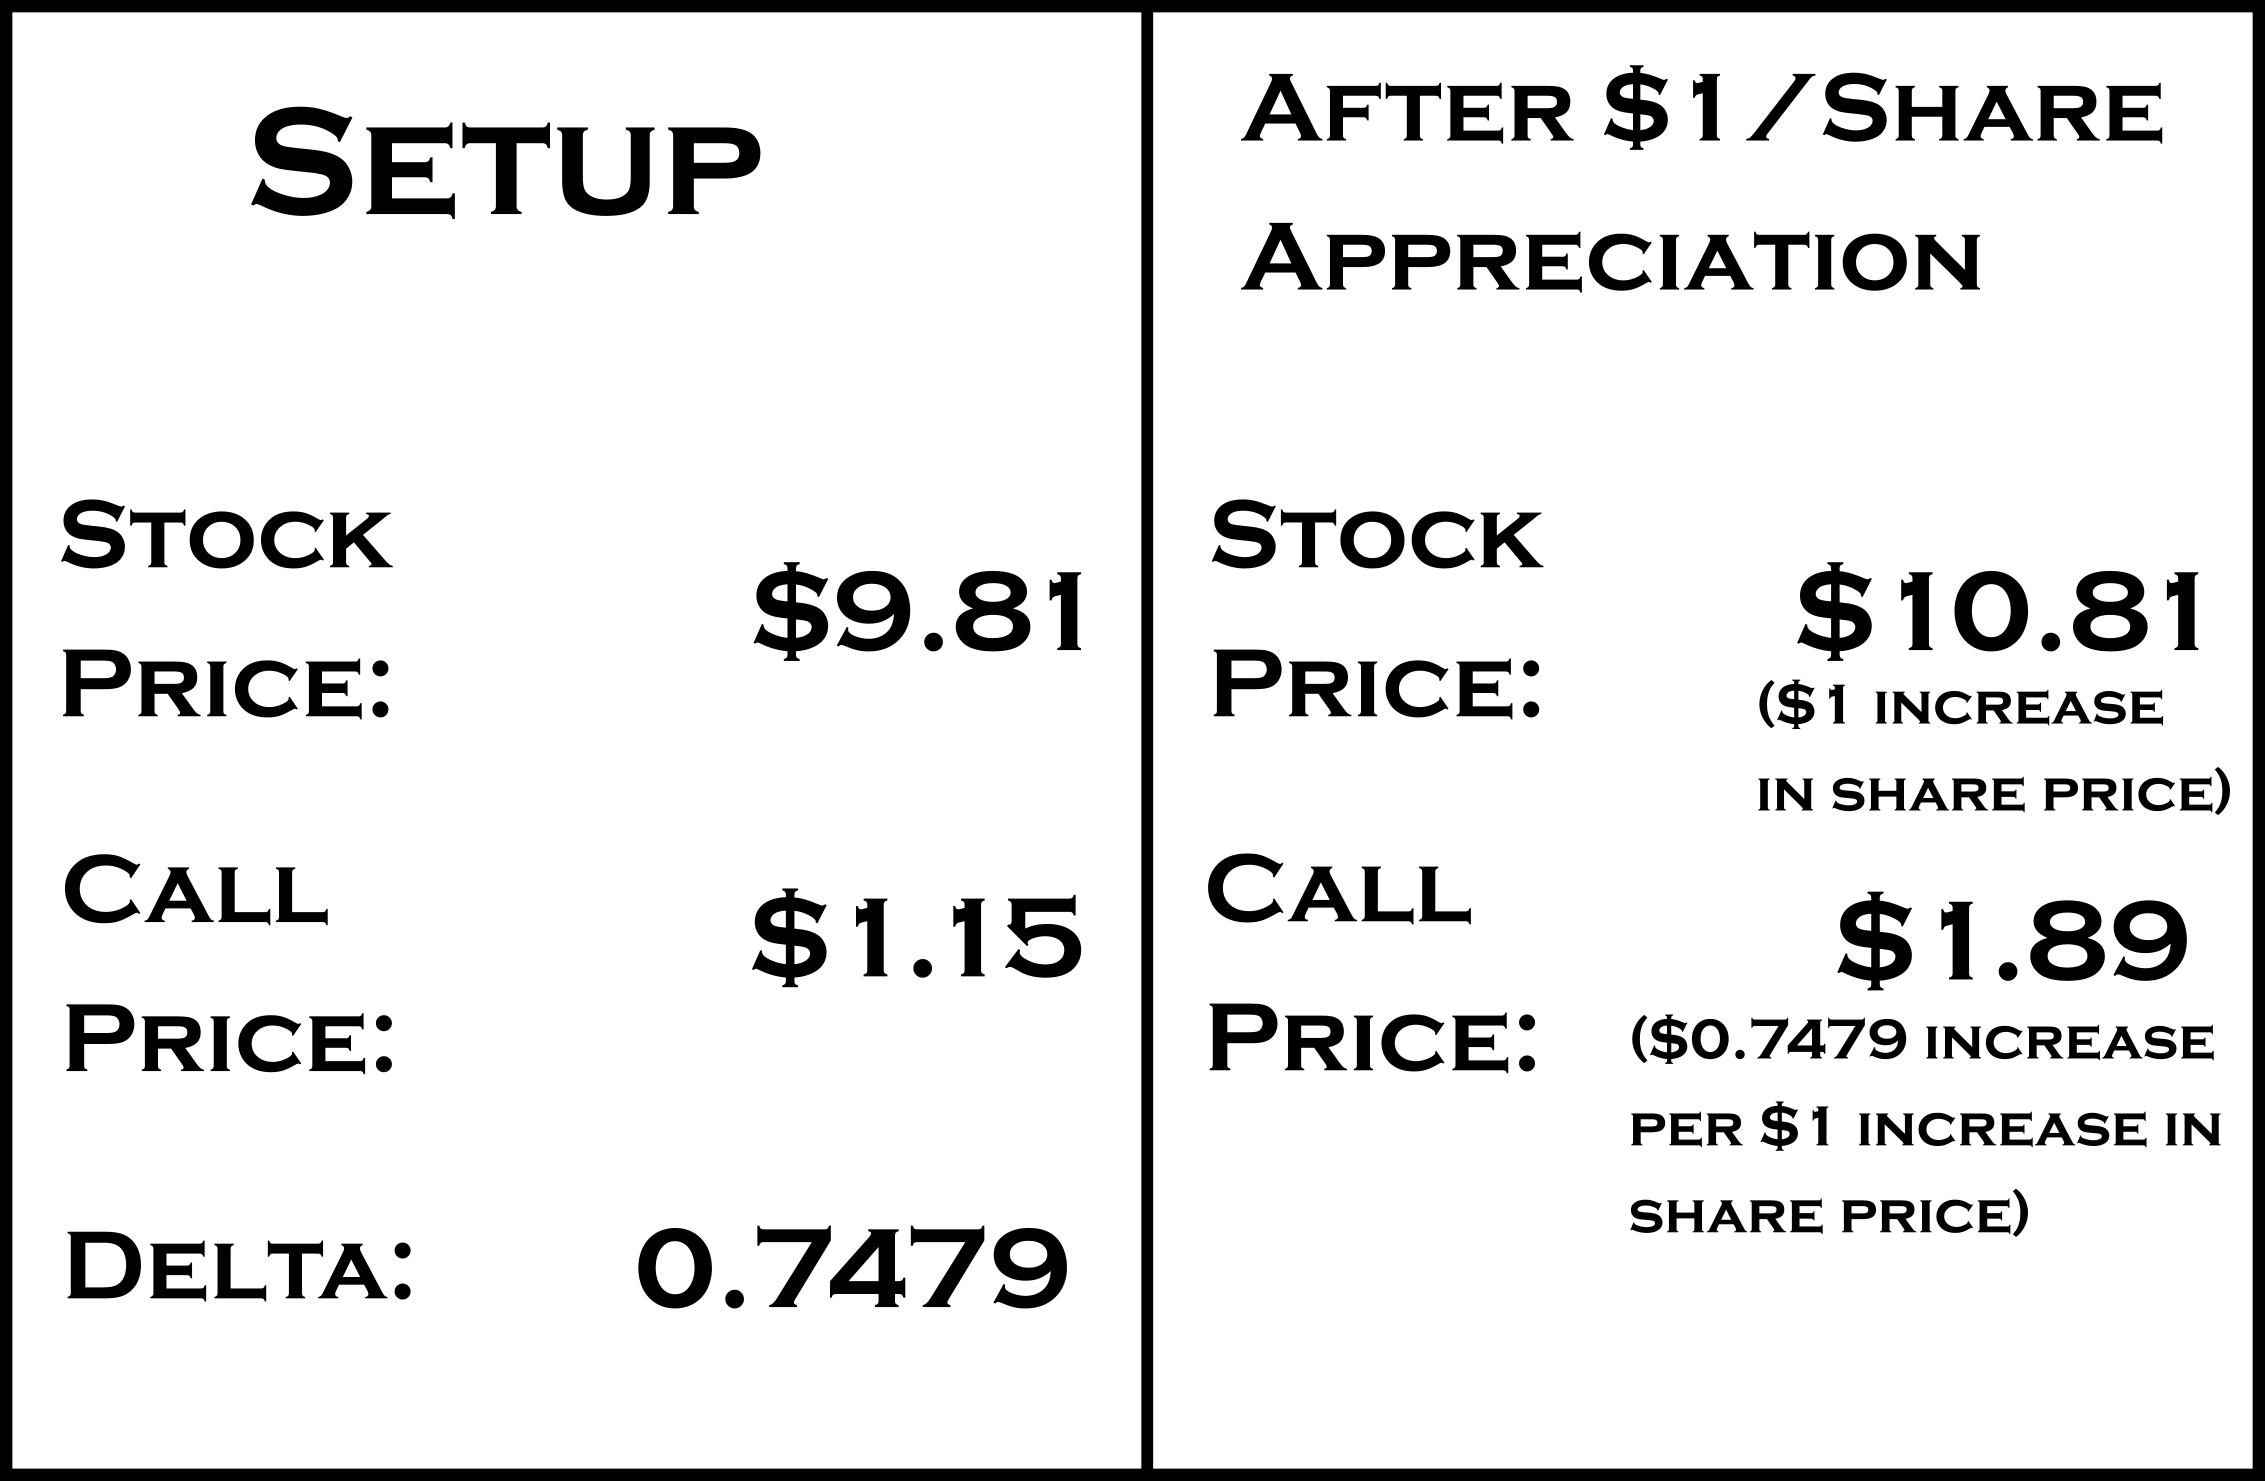
\includegraphics[width=0.85\textwidth]{Images/Ch11/chapter11pic6.png}
\end{figure}

\newpage
We should be able to generalize from these two examples that further OTM options have low deltas, and further ITM options have higher deltas. You can roughly graph the relationship of delta to moneyness, if it helps you understand better:

\begin{figure}[H]
  \centering
    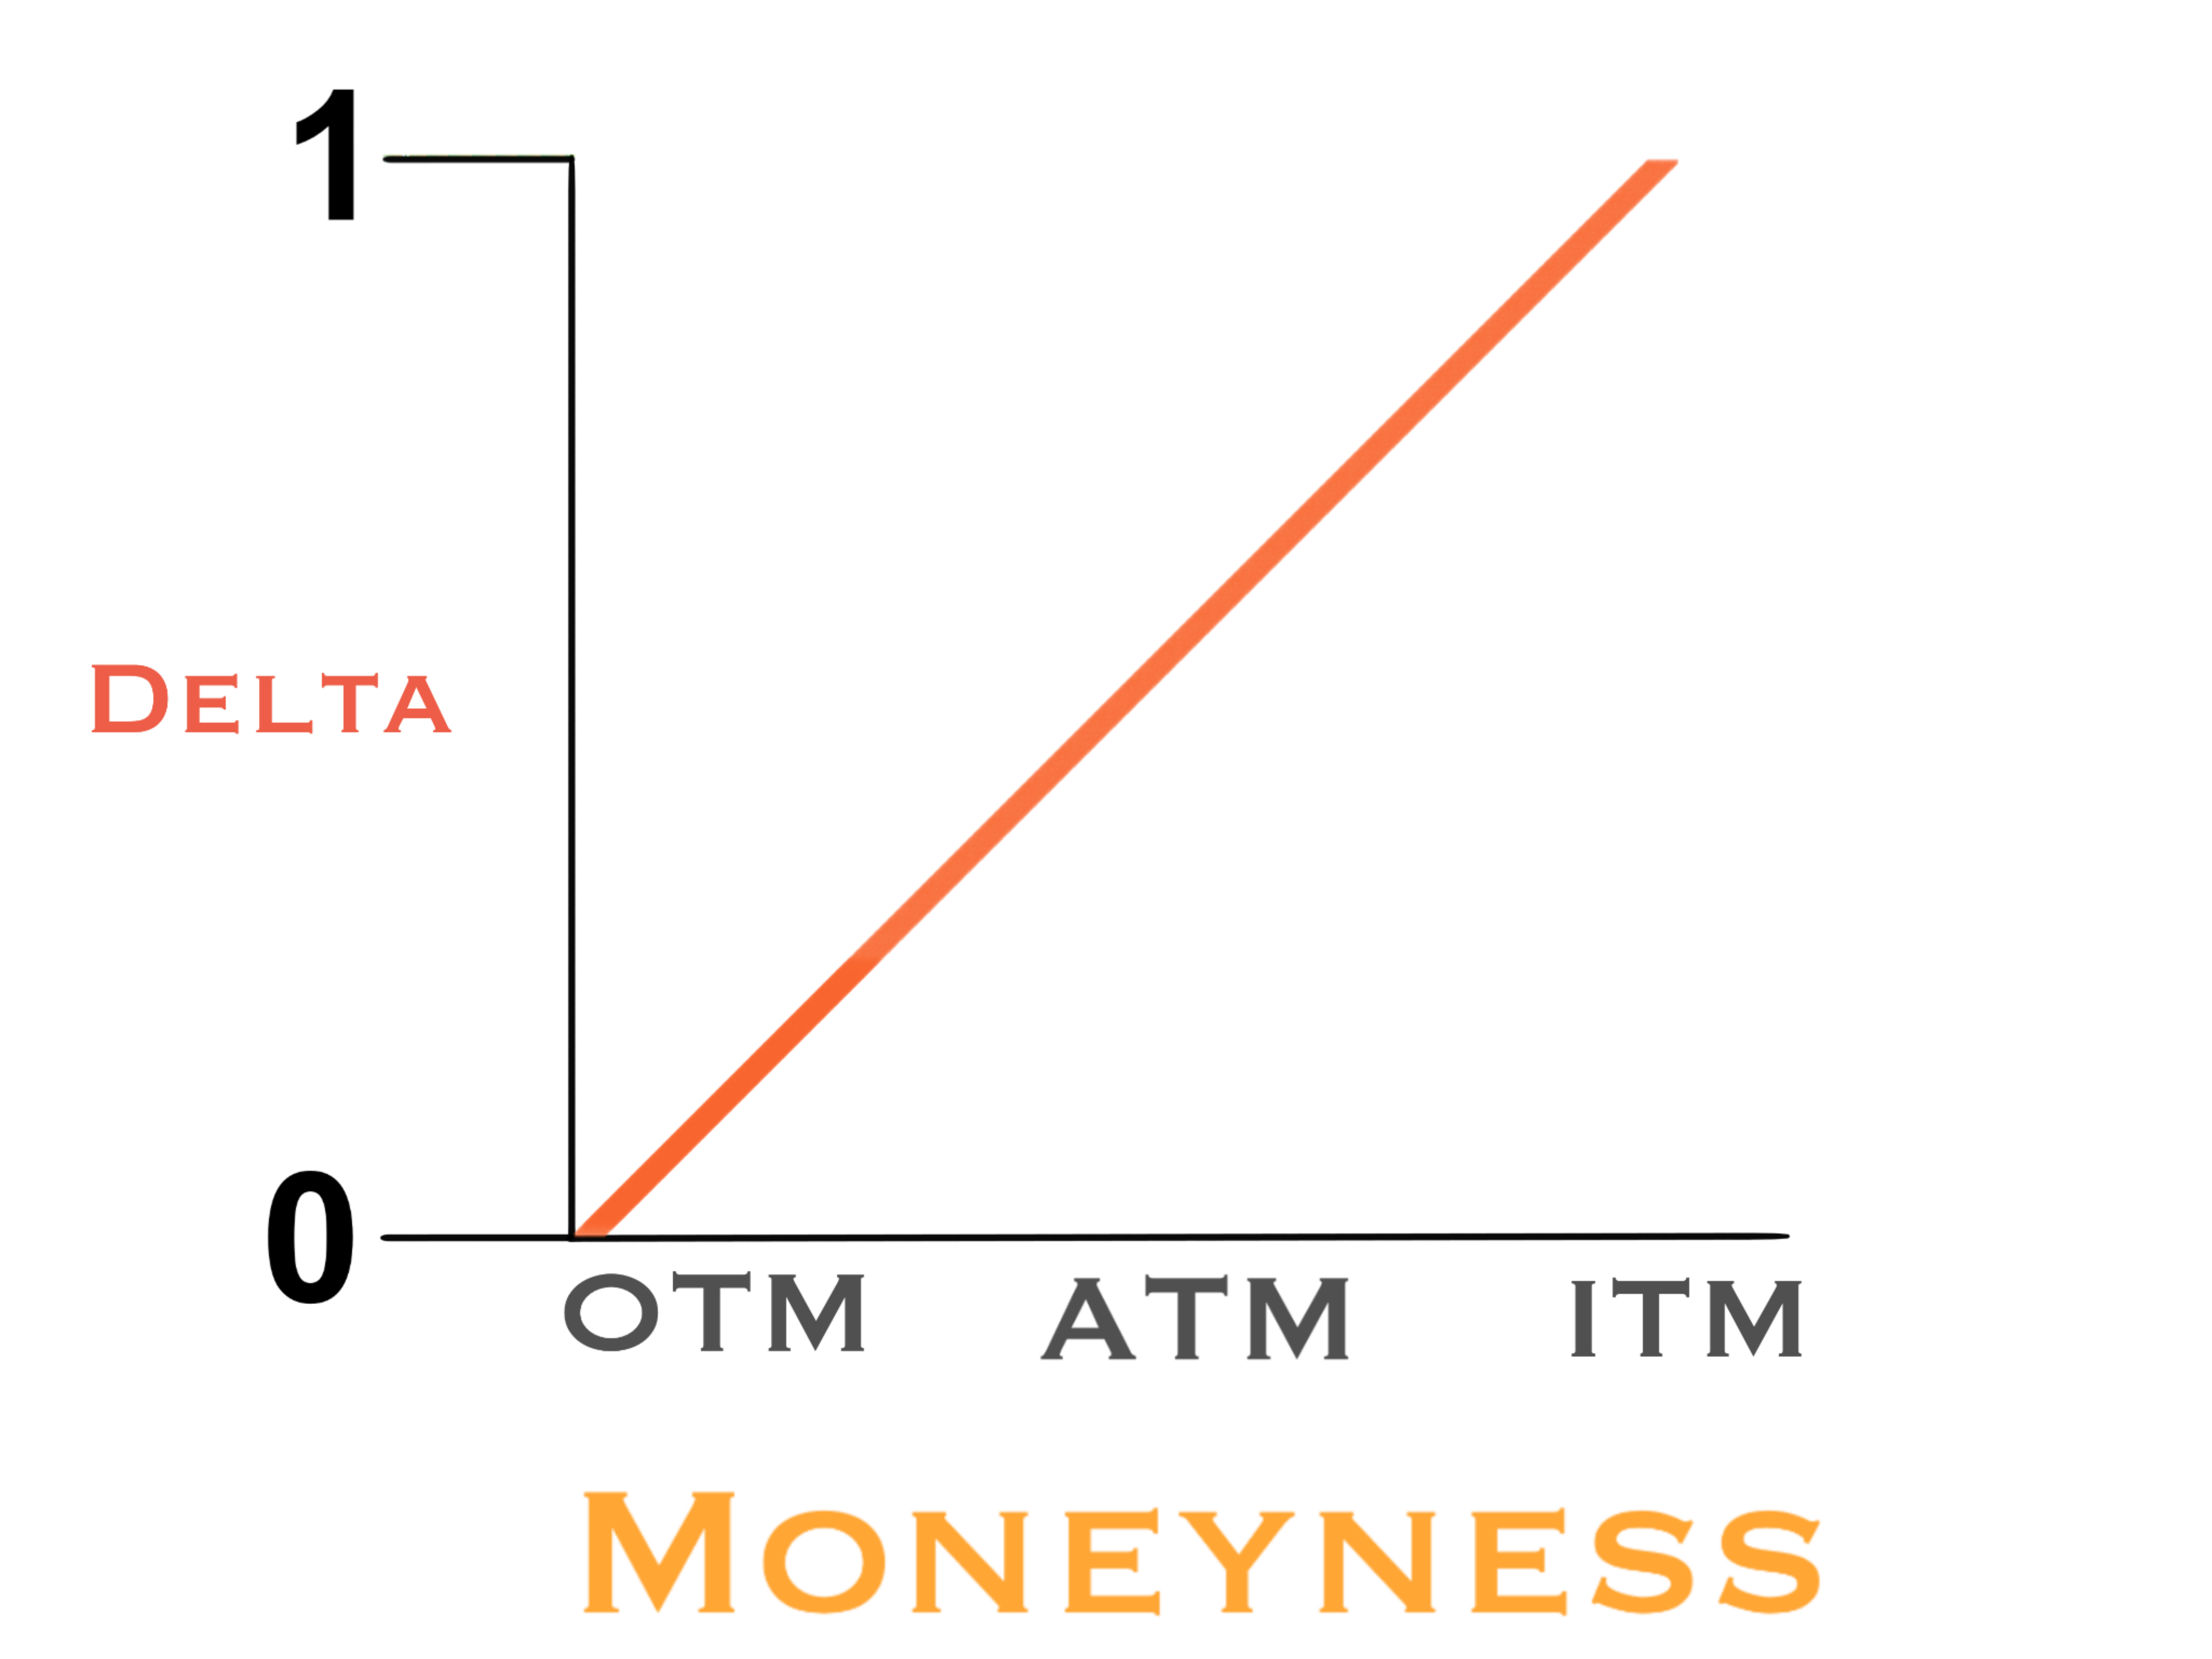
\includegraphics[width=0.7\textwidth]{Images/Ch11/chapter11pic7.png}
\end{figure}

\newpage
More precisely, it moves more like an “S” curve because delta increases exponentially as the call option becomes closer to ATM and levels off near 1 as delta goes further ITM.

\begin{figure}[h!]
  \centering
    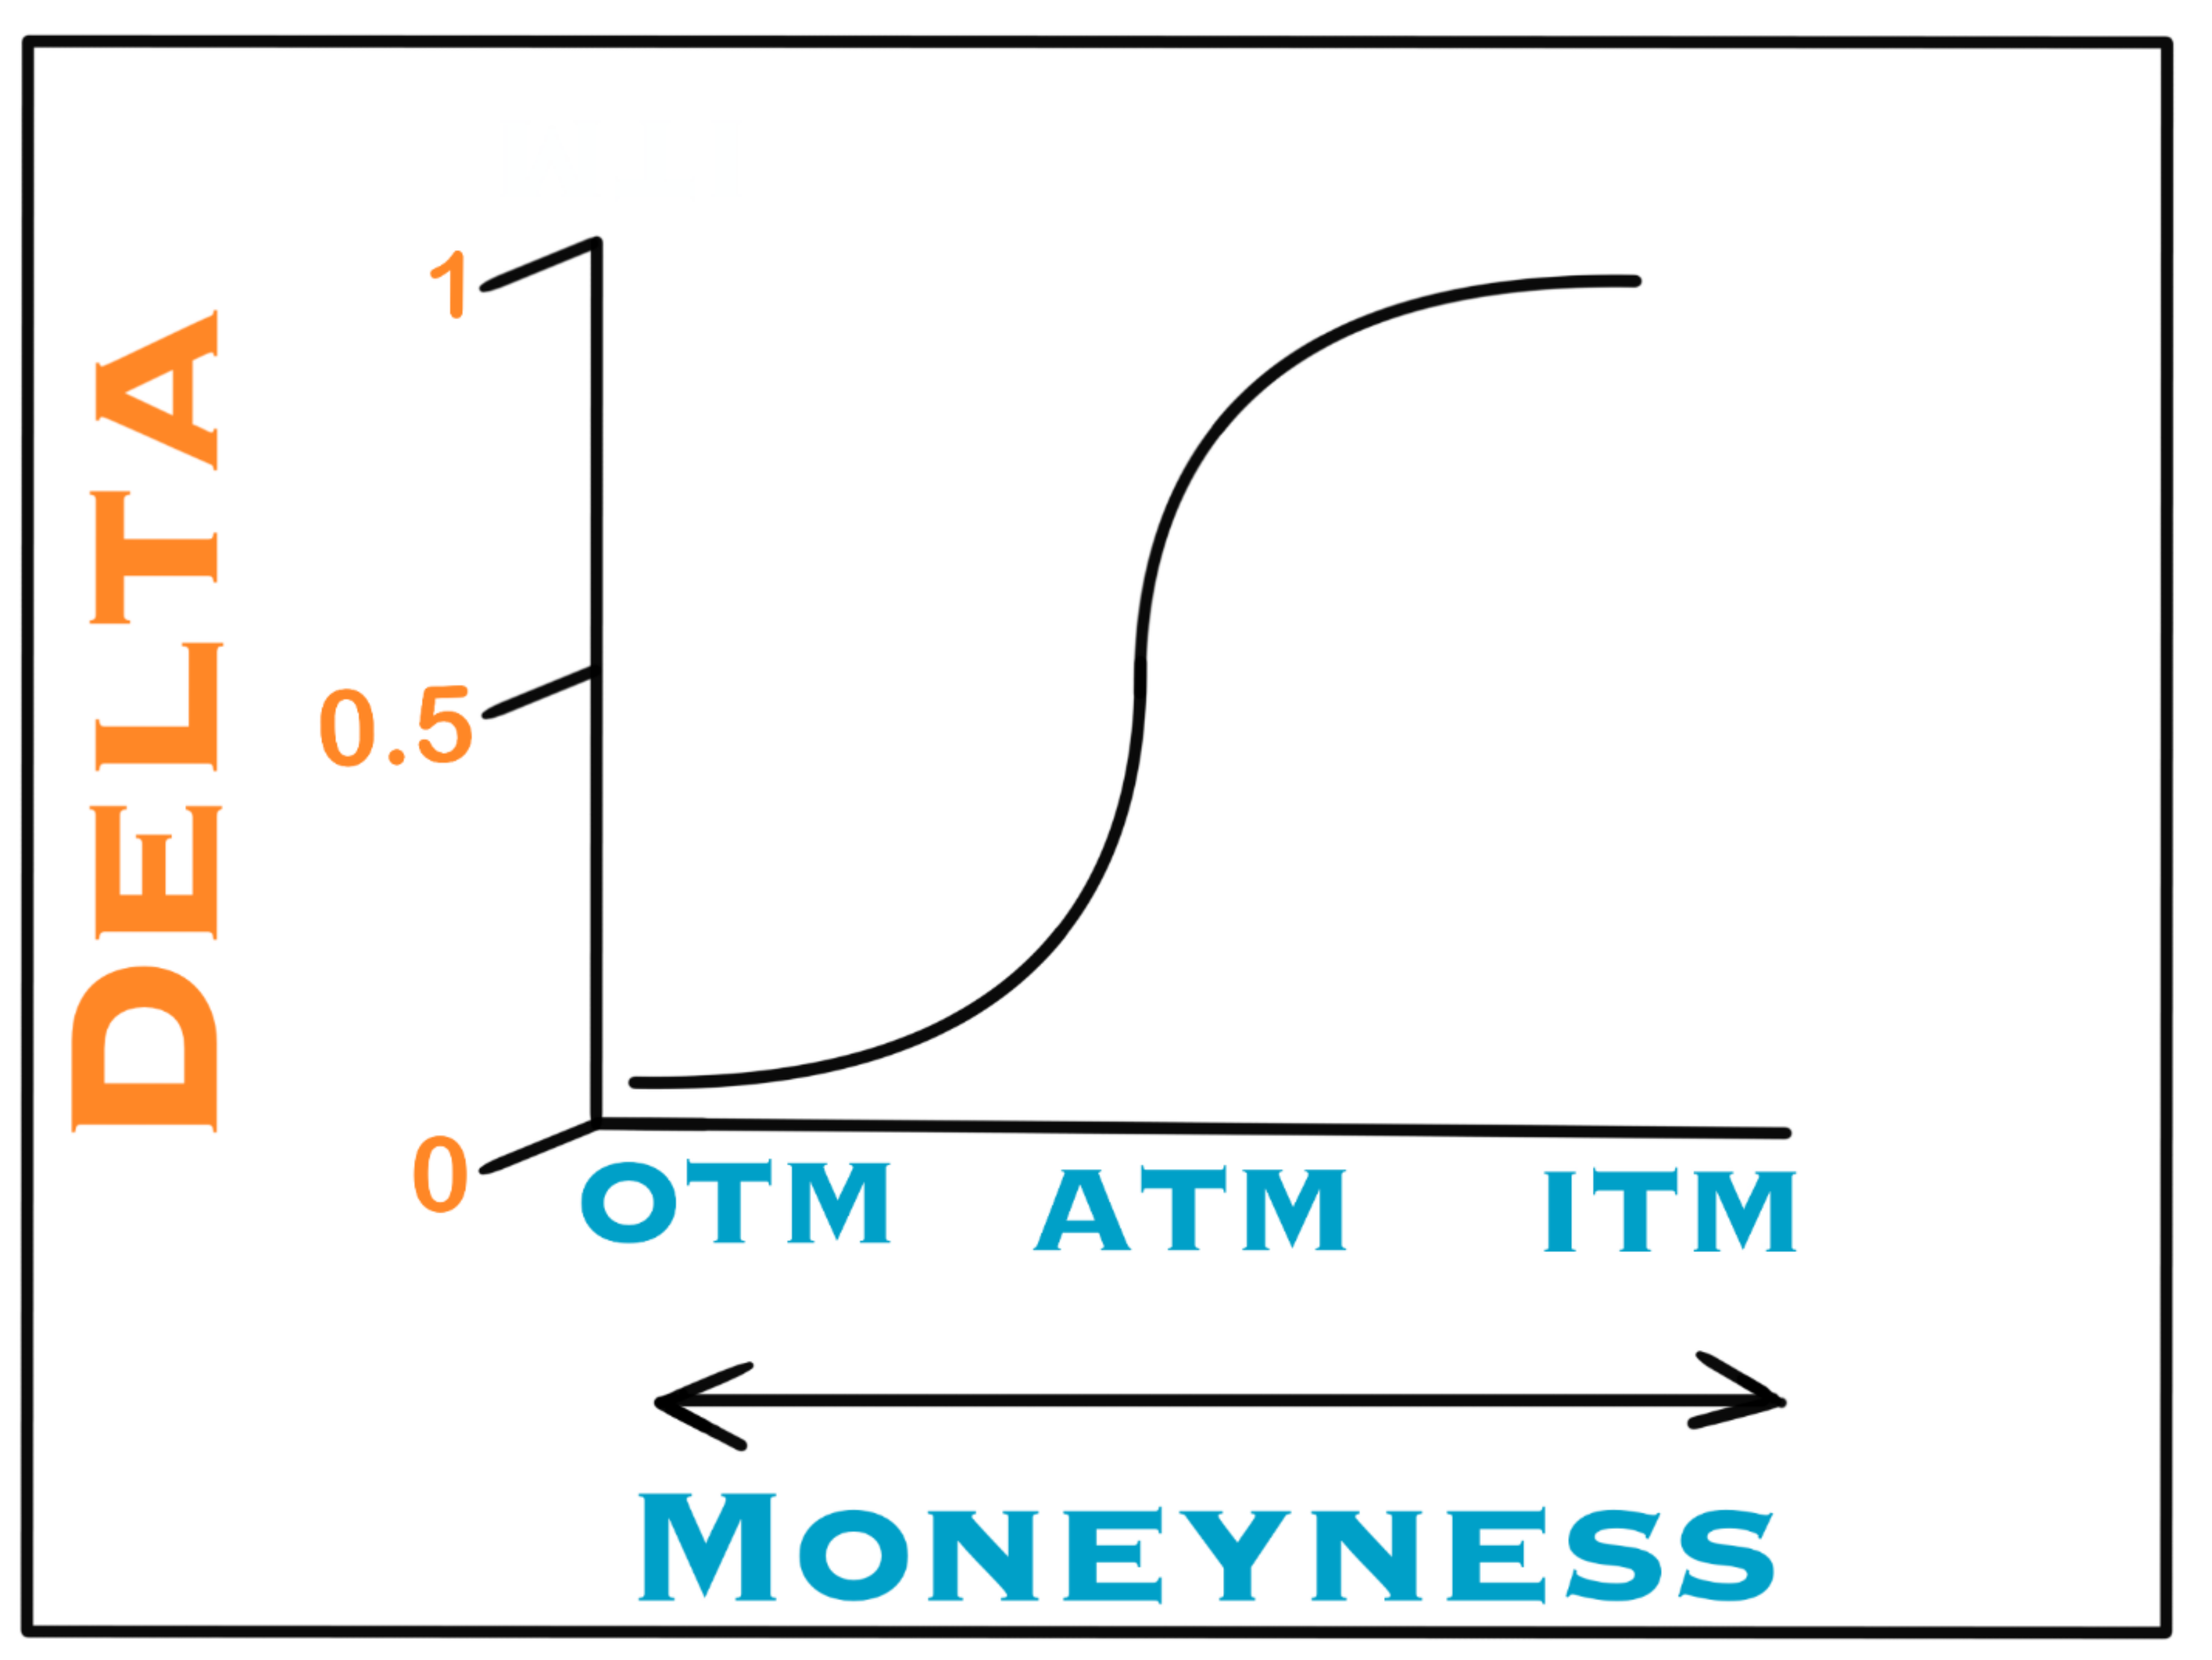
\includegraphics[width=0.7\textwidth]{Images/Ch11/chapter11pic8.png}
\end{figure}

Even better, you can pull up an options chain on your broker’s website and watch the delta change throughout the day in tandem with the stock price changes. It’s riveting.\footnote{This is serious if you find options as interesting as I do, sarcastic if you do not.} 

\newpage
\section{Bigger Uncertainty Leads to\\ Bigger Moves (and Even Bigger\\ Returns)}

The other factor influencing delta is extrinsic value/implied volatility. Right now that \$14 strike call is only trading at 5 cents because the stock is sitting at \$9.81. The chances it is going to bump up to \$14, a 42.7\% increase, in the next 26 days are probably pretty slim.\footnote{Note: if that person knows something we don’t or expects the stock to skyrocket in the meantime due to some good news, then that 5 cent option might seem like a great deal.} To put it another way, someone wanting to pay you for the right to buy a \ stock for \$14 a share might seem a bit silly, and they therefore aren’t going to pay much for that right- only 5 cents now, and only 3.78 more cents\footnote{An increase of 5 cents to 8.78 cents \emph{is a 60+\% increase.} This should raise eyebrows for investors thinking about \% returns. } if the stock goes to \$10.81. The option has a low delta, it doesn’t care much. 

But, if that stock regularly moved up and down \$6 at a time, hitting \$14 would be more probable, and someone in their right mind would pay you more than 5 cents for the right to buy it for \$14 in 26 days. Such a wildly vacillating stock price would have more implied volatility (because it is more volatile, and the increased extrinsic value would result in the price of the option premium being higher).

\newpage
\section{Extrinsic Value can be The Lion’s\\ Share}

Before we wrap it up, you have to be aware that although intrinsic value has a more concrete effect on delta, extrinsic value can represent a very significant percentage of the underlying stock’s price. This is especially true of longer-dated calls, which have more time, and therefore more time value. To illustrate this, it is helpful to compare next month's delta on the same option with the delta 789 days from now.\footnote{This longer term option is a LEAPS- Long term Equity AnticiPation Security. LEAPS function just like regular options, but they have an expiry date 1-2 years in the future.}  

First let’s look at the chain 54 days from now (recall that we were looking at a chain with expiration dates 26 days in the future previously). 

\begin{figure}[H]
  \centering
    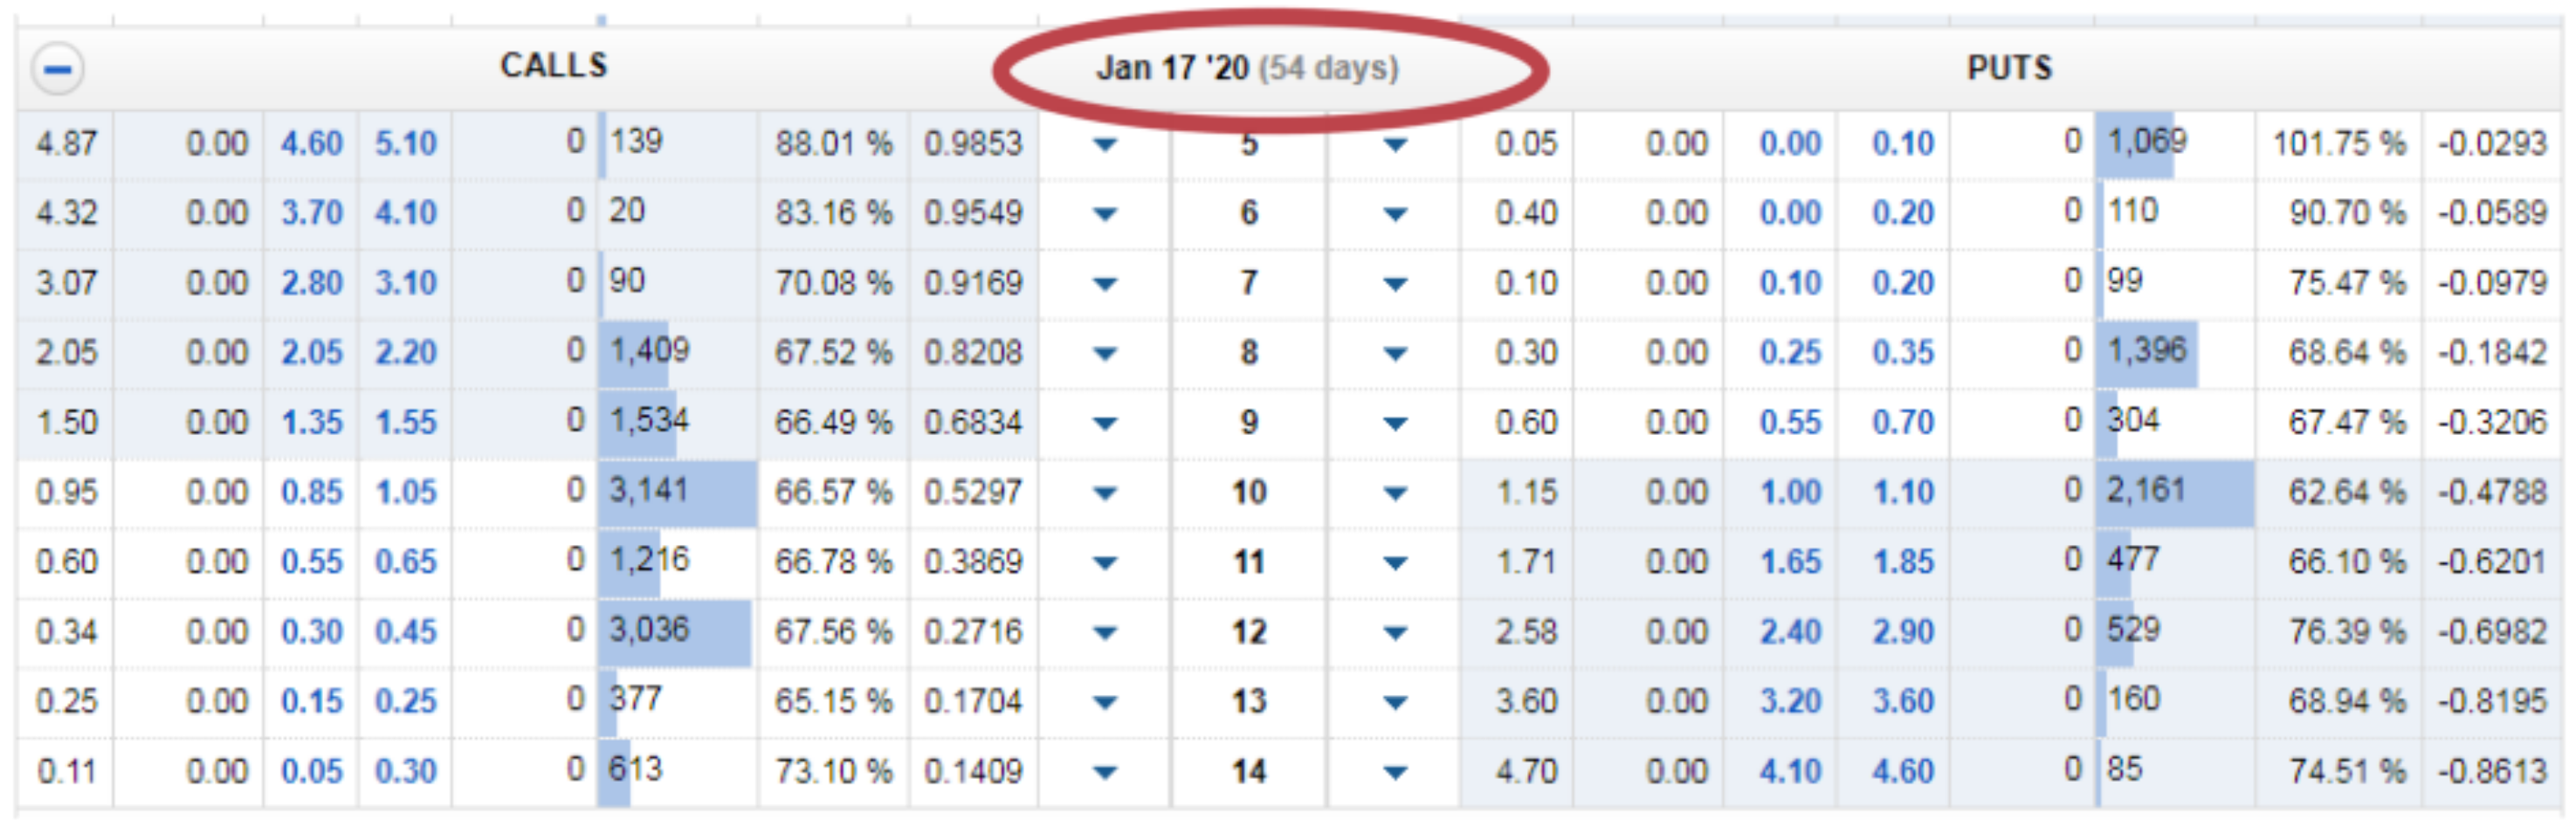
\includegraphics[width=\textwidth]{Images/Ch11/chapter11pic9.png}
\end{figure}

\newpage
Zooming in and looking at the \$10 strike Delta for 54 days from now, notice it went from 0.4987 in the previous chain to 0.5297- a bit of a bump (I intentionally didn’t circle the value so you could practice finding it).

\begin{figure}[H]
  \centering
    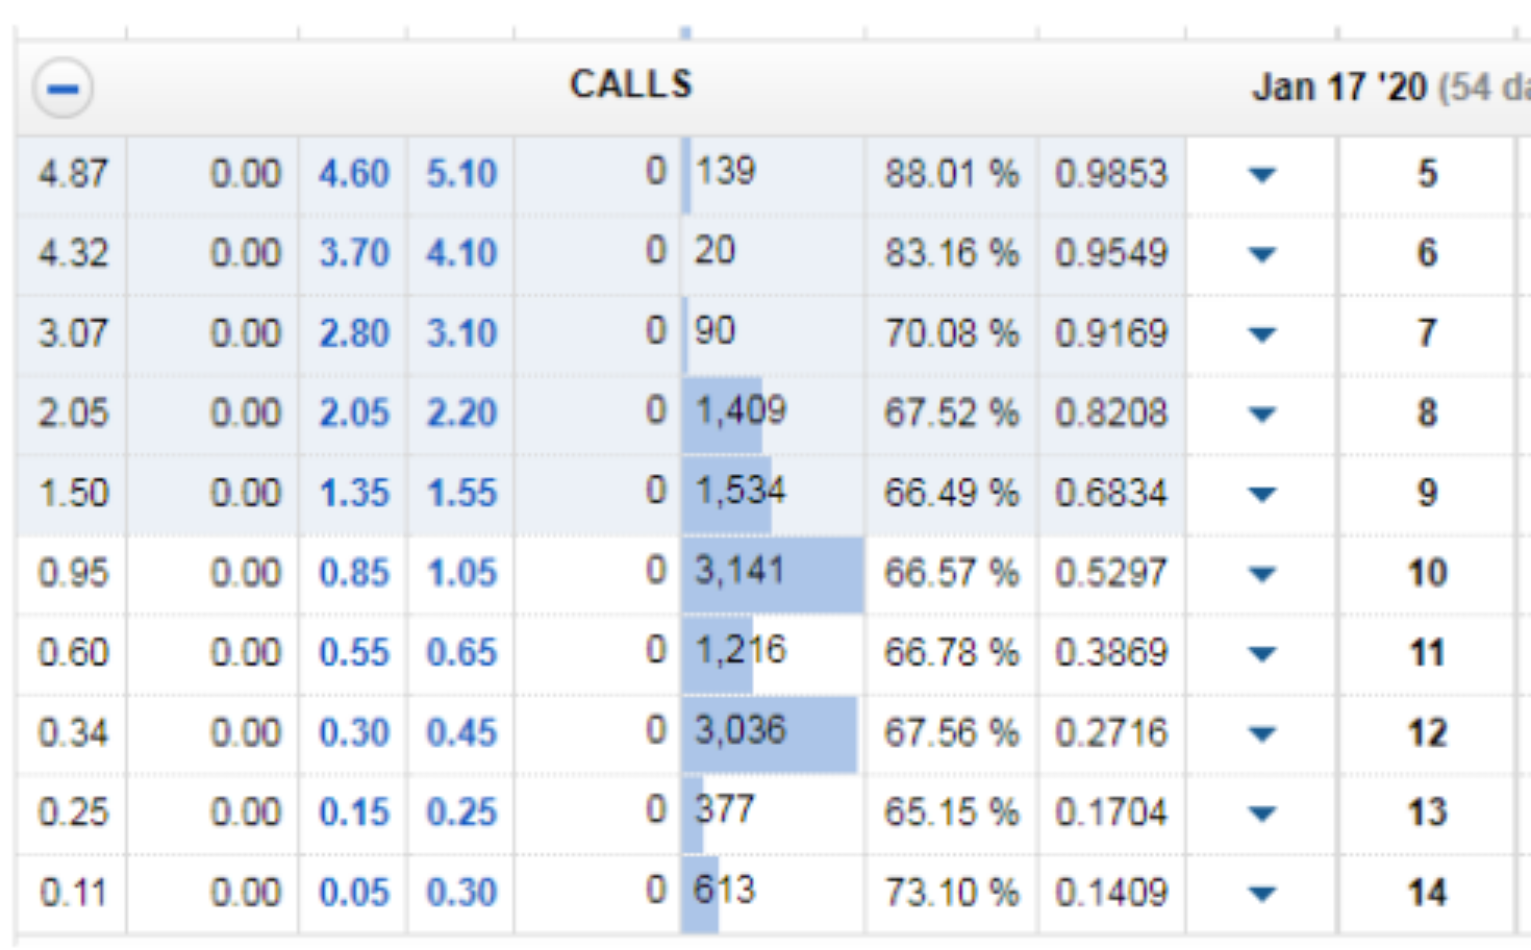
\includegraphics[width=\textwidth]{Images/Ch11/chapter11pic10.png}
\end{figure}


Now let’s compare the 54-day call to the two-year LEAP...

\begin{figure}[H]
  \centering
    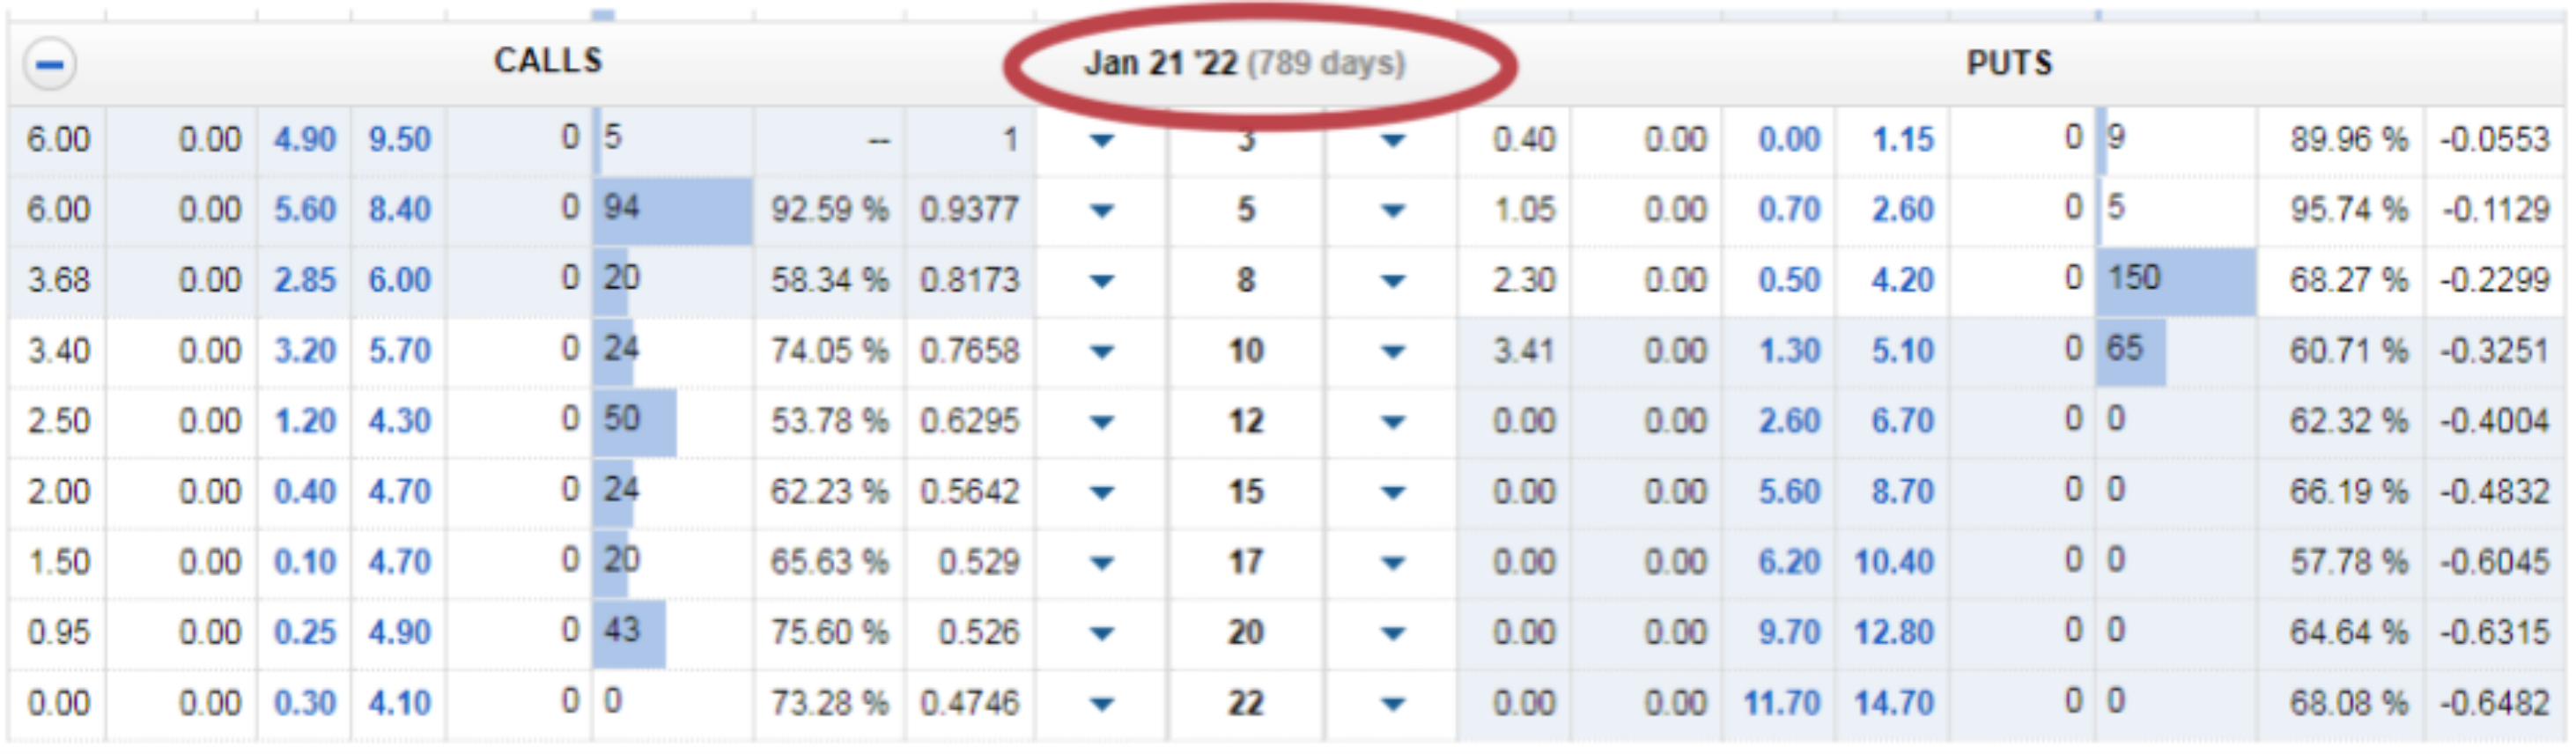
\includegraphics[width=\textwidth]{Images/Ch11/chapter11pic11.png}
\end{figure}

\newpage
Looking at the \$10 strike Delta for 789 days from now, notice it is 0.7658- a big bump from 0.4987.

\begin{figure}[H]
  \centering
    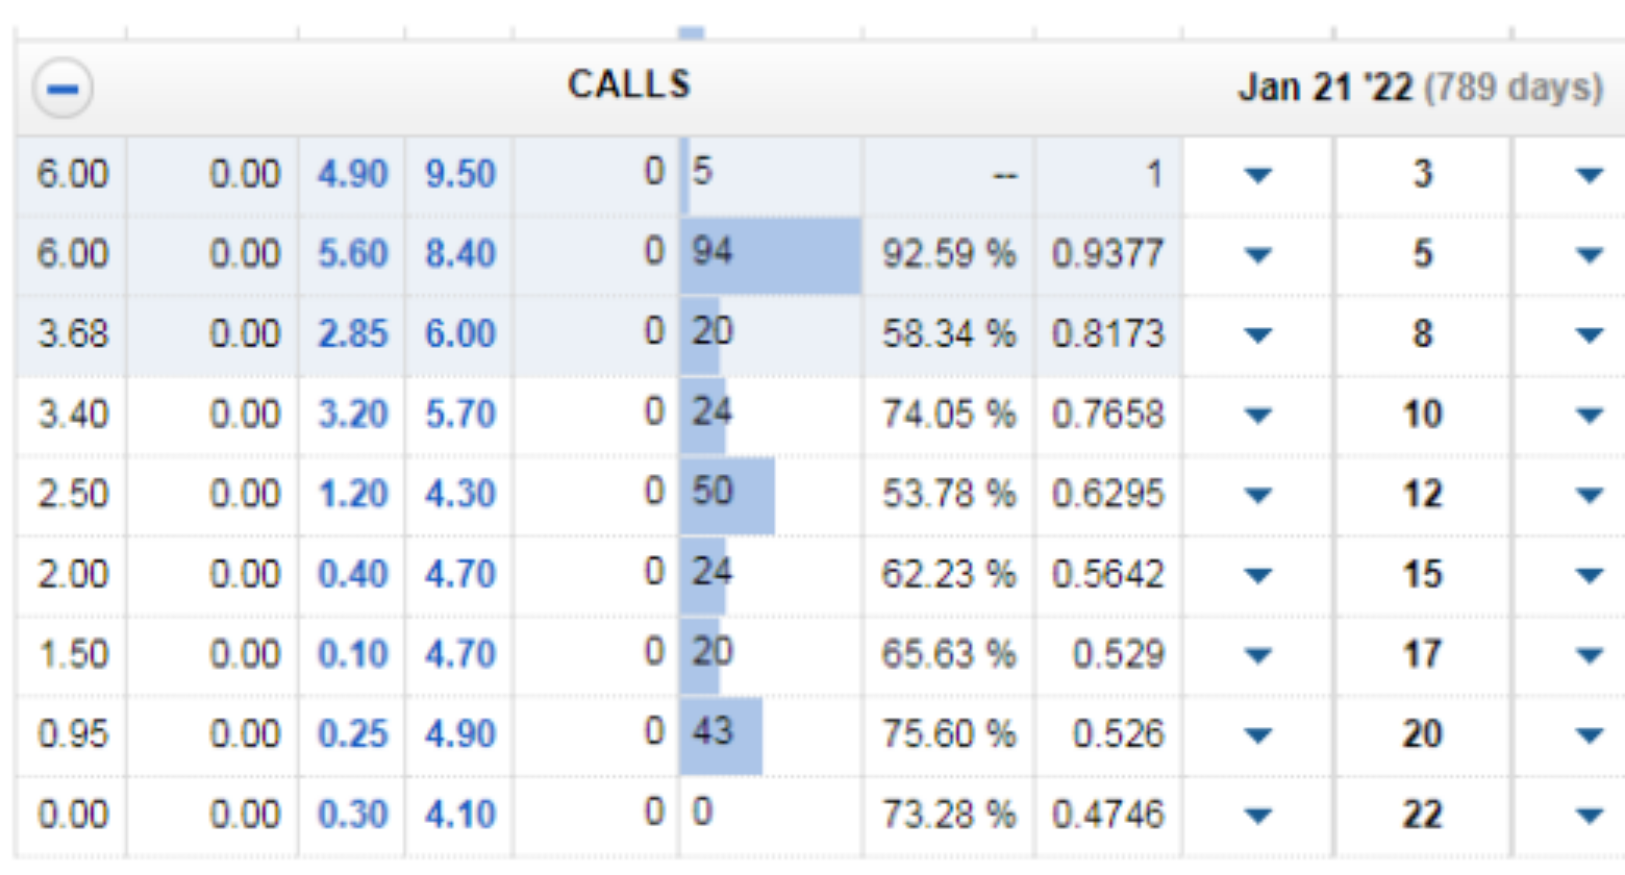
\includegraphics[width=\textwidth]{Images/Ch11/chapter11pic12.png}
\end{figure}

This happened because delta is tied to option value, which is inherently composed of intrinsic and extrinsic value. A lot can happen in 2 years. \textbf{A LOT.} A company can go bankrupt or discover a cure for hemophilia- so that extra time translates to a lot of time value. Extrinsic value is, inherently, the value of the unknowns in play for any given stock.


\section{34\% Return in Two Years?}

If you reflect on this a bit, it seems like a good idea to buy a stock for \$9.81 a share, then sell someone the right to buy it from you for \$10 a share. In the above chain, that right just sold for \$3.40 a share, so you’d make 36\% on your investment in 2 years if the price went up, and you’d break even if the price dropped to \$6.4- protection of 34\% to the downside! Seems like a good deal, this selling LEAPs thing. But as with most things in life, it's more complicated than that. 

Do you know for sure you want to own any given stock for 2 years?\footnote{If you are a Boglehead, the answer is a resounding yes for your chosen indexes.}  Can you stick to your plan for 2 years and not be wracked with regret if the stock jumps to \$20 (or \$50) a share? More on that later, but for now we need to clarify that delta is a moving target, and then go over some cool tricks with delta to help you understand it better if you want a deeper intuition. Then we’ll finally get to the topic of time value.